\section{Konzeption}
Das Modul Mimikry setzt ein gezieltes, IT gestütztes Training zum Ausgleich der Defizite im  Bereich von Ausdrücken von Emotionen um das Ausdrücken der Emotionen ist eine soziale Kompetenz, die durch Stärkung der Mimikry Fähigkeit, also einen Ausgleich der bereits existierenden Defizite, weiterentwickelt werden kann. Das Konzept des Mimikry Moduls wurde auf Basis eines Entwurf entwickelt, der in Kooperation mit einem Team aus Psychologen der Humboldt Universität und einer Designerin für das Projekt EMOTISK entstand. Dieser Entwurf bestand aus einer Sammlung von Grafiken die mögliche Screens der App zu fünf Mimikry Szenarien dargestellt haben. 
Im Mittelpunkt des Konzeptes des Mimikry Moduls steht der Erwerb von Kompetenzen, die dem Nutzer helfen, das richtige (und situativ angemessene) Ausdrücken von Gesichtsausdrücken zu beherrschen. Diese Übertragbarkeit wurde in anderen aktuellen Projekten noch nicht ausreichend untersucht und stellt daher eine Lücke dar, die noch zu erforschen gilt. 
Im Rahmen dieser Bachelorarbeit sollte die Eignung eines IT-gestützten Trainings experimentell erforscht werden. Diese Eignung entspricht daher weder dem therapeutischen Zweck noch der Wirksamkeit des Trainings sondern der Gebrauchstauglichkeit zum IT-gestützten Training. Der Entwurf bestand aus fünf Aufgabetypen, mir wurde die Entscheidung überlassen, welche und wie viel umgesetzt werden. Es wurden zwei der fünf Varianten implementiert und evaluiert - eine mit Kameravorschau und eine ohne Kameravorschau. 
\subsection{Beschreibung des Konzepts Mimikry Moduls}
In dem Mimikry Modul aus der E.V.A. App werden dem Benutzer emotionale Gesichtsausdrücke präsentiert, die von ihm nachgemacht werden müssen. Die Nachahmung wird aufgenommen und mit der SHORE\re Software zur Gesichtserkennung direkt ausgewertet, siehe Kapitel 2, Grundlagen, Zusammenarbeit mit dem Fraunhofer Institut - SHORE\re.
\subsection{Konzeptionellen Entscheidungen}
Für den Zweck dieser Bachelorarbeit wurden zwei der fünf existierenden Mimikry Varianten für die Implementierung ausgewählt, Mimikry III und Mimikry IV. 
Bei der ersten Variante wird der Benutzer aufgenommen, die Aufnahme wird auf dem Bildschirm direkt angezeigt. Bei der zweiten Variante wird auch eine Aufnahme betätigt, es wird jedoch keine Vorschau angezeigt. Die Varianten wurden zur Mimikry I und Mimikry II umbenannt, um die Verwirrung zu vermeiden. 

\subsection{Beschreibung des entworfenen Mimikry Moduls}
Basierend auf dem zur Verfügung gestellten Design und des bisher gesammelten Wissen, wurden folgenden Entscheidungen zum Verlauf des Mimikry Spiels getroffen.

Vor dem ersten Spielen der Mimikry Varianten wird eine Einführung auf dem Bildschirm angezeigt. Zu Beginn der beiden Spielaufgaben wird eine Zielemotion zufällig ausgewählt, siehe Abb. \ref{mit_diagramm}. Es existieren vier möglichen Grundemotionen: Heiter, Ärgerlich, Überrascht und Traurig, die nachzuahmen sind. Der Spielers sollte die vorgegebene Zielemotion mit eigenen Gesichtsausdrücken für eine bestimmte Zeit imitieren vgl. Abbildung \ref{mit} und \ref{ohne}. Nach Ablauf der Zeit bekommt der Spieler ein neuer Screen angezeigt. Auf diesem Screen wird ihm vermittelt, ob die Aufgabe richtig oder falsch gelöst wurde. Die Meldungen wurden so konzipiert, dass sind in einer freundlichen und unterstützenden Form gehalten werden. Es sollte als motivierender Faktor wirken.
Der Verlauf des Spiels besteht aus folgenden Schritten:

\begin{enumerate}
    \item Einführung in die Übung.
    \item Das Generieren und anzeigen einer Emotion, die der Nutzer nachmachen sollte.
    \item Je nach dem Spielszenario wird eine Kamera Vorschau verfügbar oder nicht. 
    \item Der Spieler sollte die vorher angezeigte Emotion  15 Sekunden lang imitieren
    \item Die Verbliebene Zeit wird dynamisch mittels eines Balkens abgebildet
    \item Wenn innerhalb der vorgegebenen Zeit mind. 75\% Korrektheit des Imitierens einer Zielemotion erreicht wurde, wird die Aufgabe als korrekt gelöst markiert.
    \item Dem Benutzer wird konstruktives Feedback angezeigt.
\end{enumerate}

\subsubsection{Mimikry I} 
Bei der Mimikry mit Vorschau werden die Zielemotionen gleichzeitig zum Erscheinen der Zielaufgabe selbst präsentiert

\begin{figure}[!ht]
\centering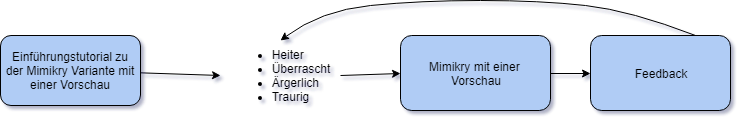
\includegraphics[width=360pt]{texes/implementierung_mimikry_preview.png}
\caption{Ablauf von Mimikry: Tutorial, Auswahl der Zielemotion durch das Spiel, Lösen der Aufgabe und Feedback. Die Auswahl der Zielemotion erfolgt vor dem Anfang der Aufgabe, wird jedoch erst während der Aufgabe selbst vermittelt.}
\label{mit_diagramm}
\end{figure}
Die Aufnahme aus der Kamera wird während der Spielphase angezeigt. Siehe Abb.\ref{mit}
\begin{figure}[!ht]
\centering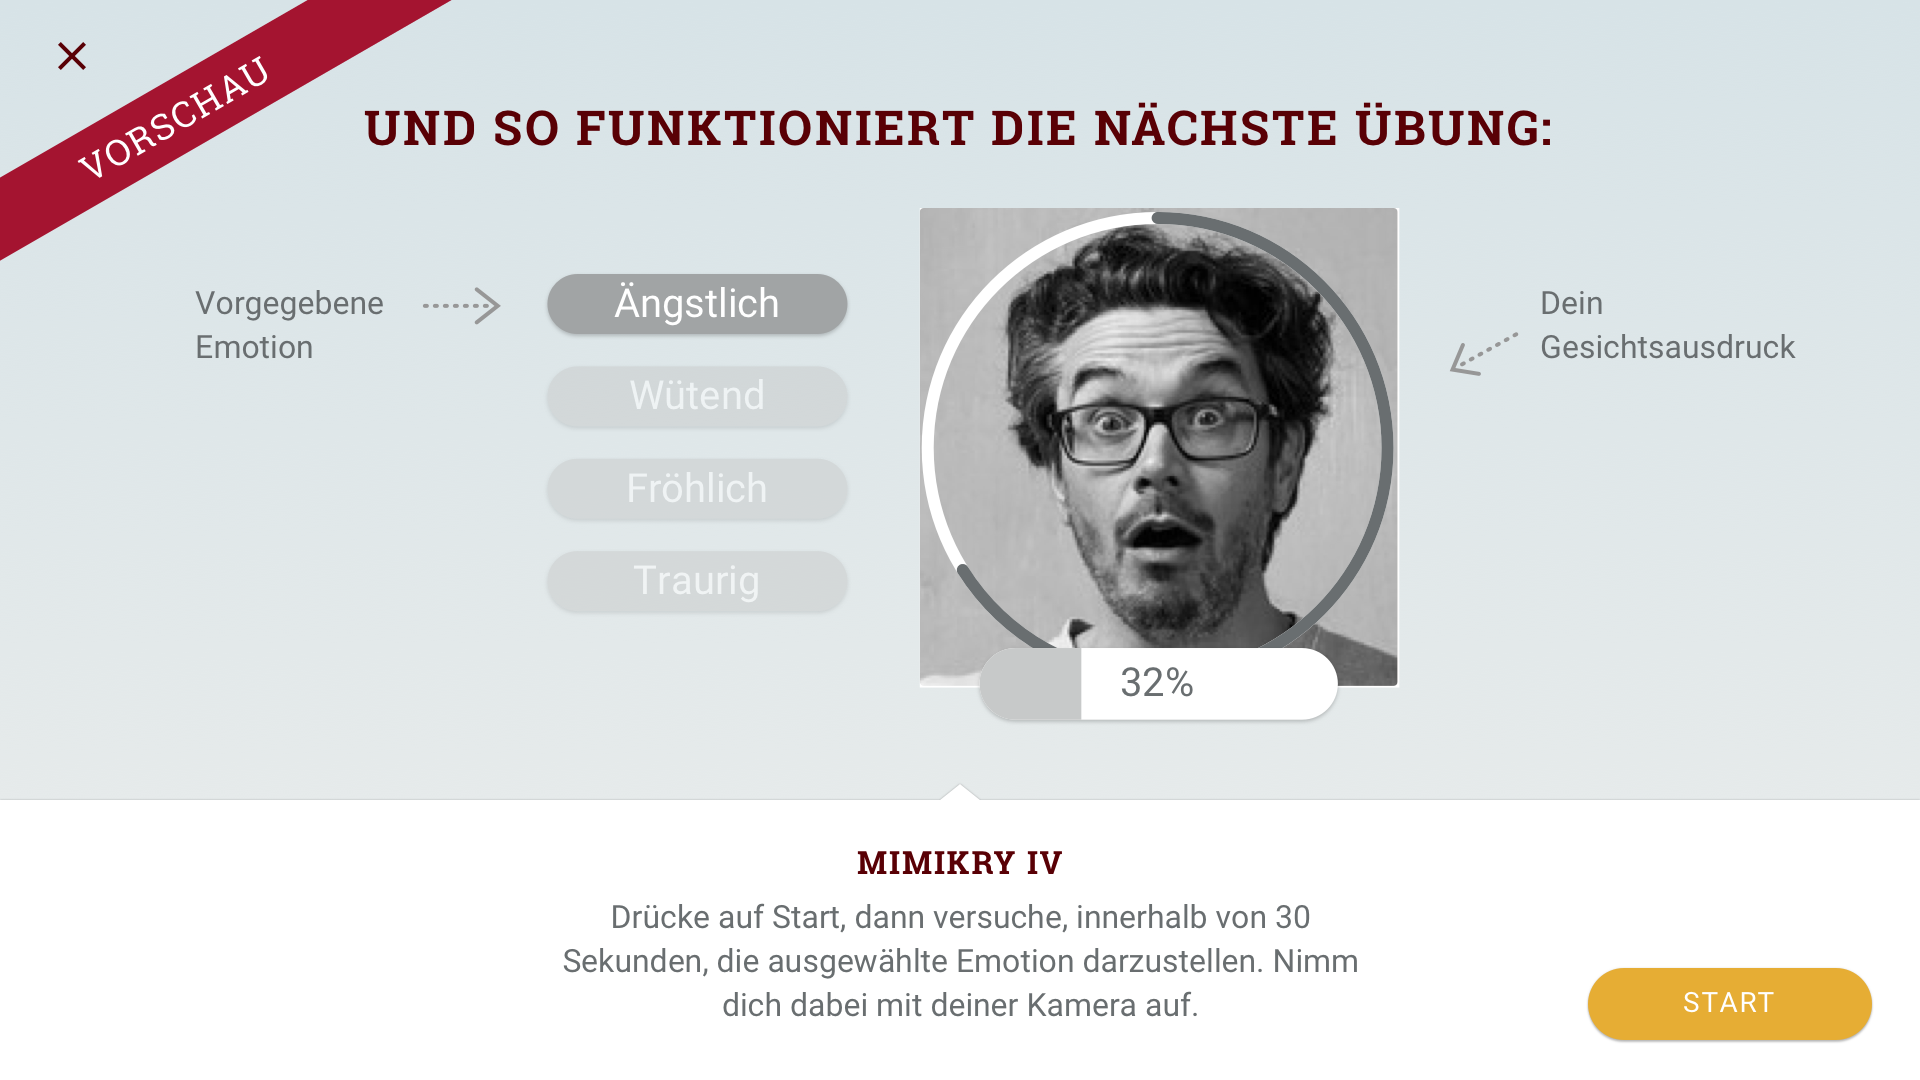
\includegraphics[width=330pt]{res/TASK_MIMIKRY_IV_INTRO.png}
\caption{Einführung des Mimikry mit Vorschau Moduls (das ursprüngliche Mimikry IV, wurde während der Implementierung zu Mimikry I umbenannt). Auf dem Bild befinden sich vier Felder mit Grundemotionen, eine der Emotionen, die Zielemotion wird vorgegeben und hervorgehoben. Auf der rechten Seite wird ein Kamerafeld innerhalb von einem runden Balken zu sehen. Darunter befindet sich ein horizontaler, länglicher Balken, der den gegenwärtigen Fortschritt abbilden soll. Die Balken wurden an der Stelle ohne Erklärungspfeilen angezeigt.}
\label{mit}
\end{figure}
\newpage
\subsubsection{Mimikry II}
Bei der Mimikry ohne Vorschau Variante wird die Zielemotion vor dem Erscheinen der Spielaufgabe selbst als ein separates Screen für 10 Sekunden präsentiert, siehe Abb.\ref{ohne_diagramm}.
\begin{figure}[!ht]
\centering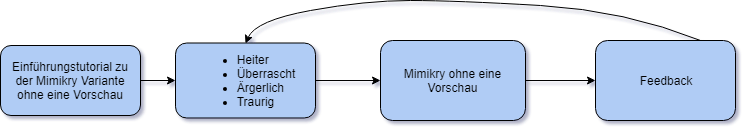
\includegraphics[width=360pt]{texes/implementierung_mimikry_no_preview.png}
\caption{Ablauf des Mimikry-Minispiel: Tutorial, Auswahl der Zielemotion durch das Spiel, Lösen der Augabe und Feedback. Die Auswahl der Zielemotion erfolgt vor dem Anfang der Aufgabe und wird dem Benutzer auf einem separaten Screen vermittelt.}
\label{ohne_diagramm}
\end{figure}
Das Ziel der Aufgabe ist identisch zur Mimikry mit Vorschau.Das Ziel gleich, allerdings wird keine Aufnahme des Gesichts angezeigt. Siehe Abb. \ref{ohne}
\begin{figure}[!ht]
\centering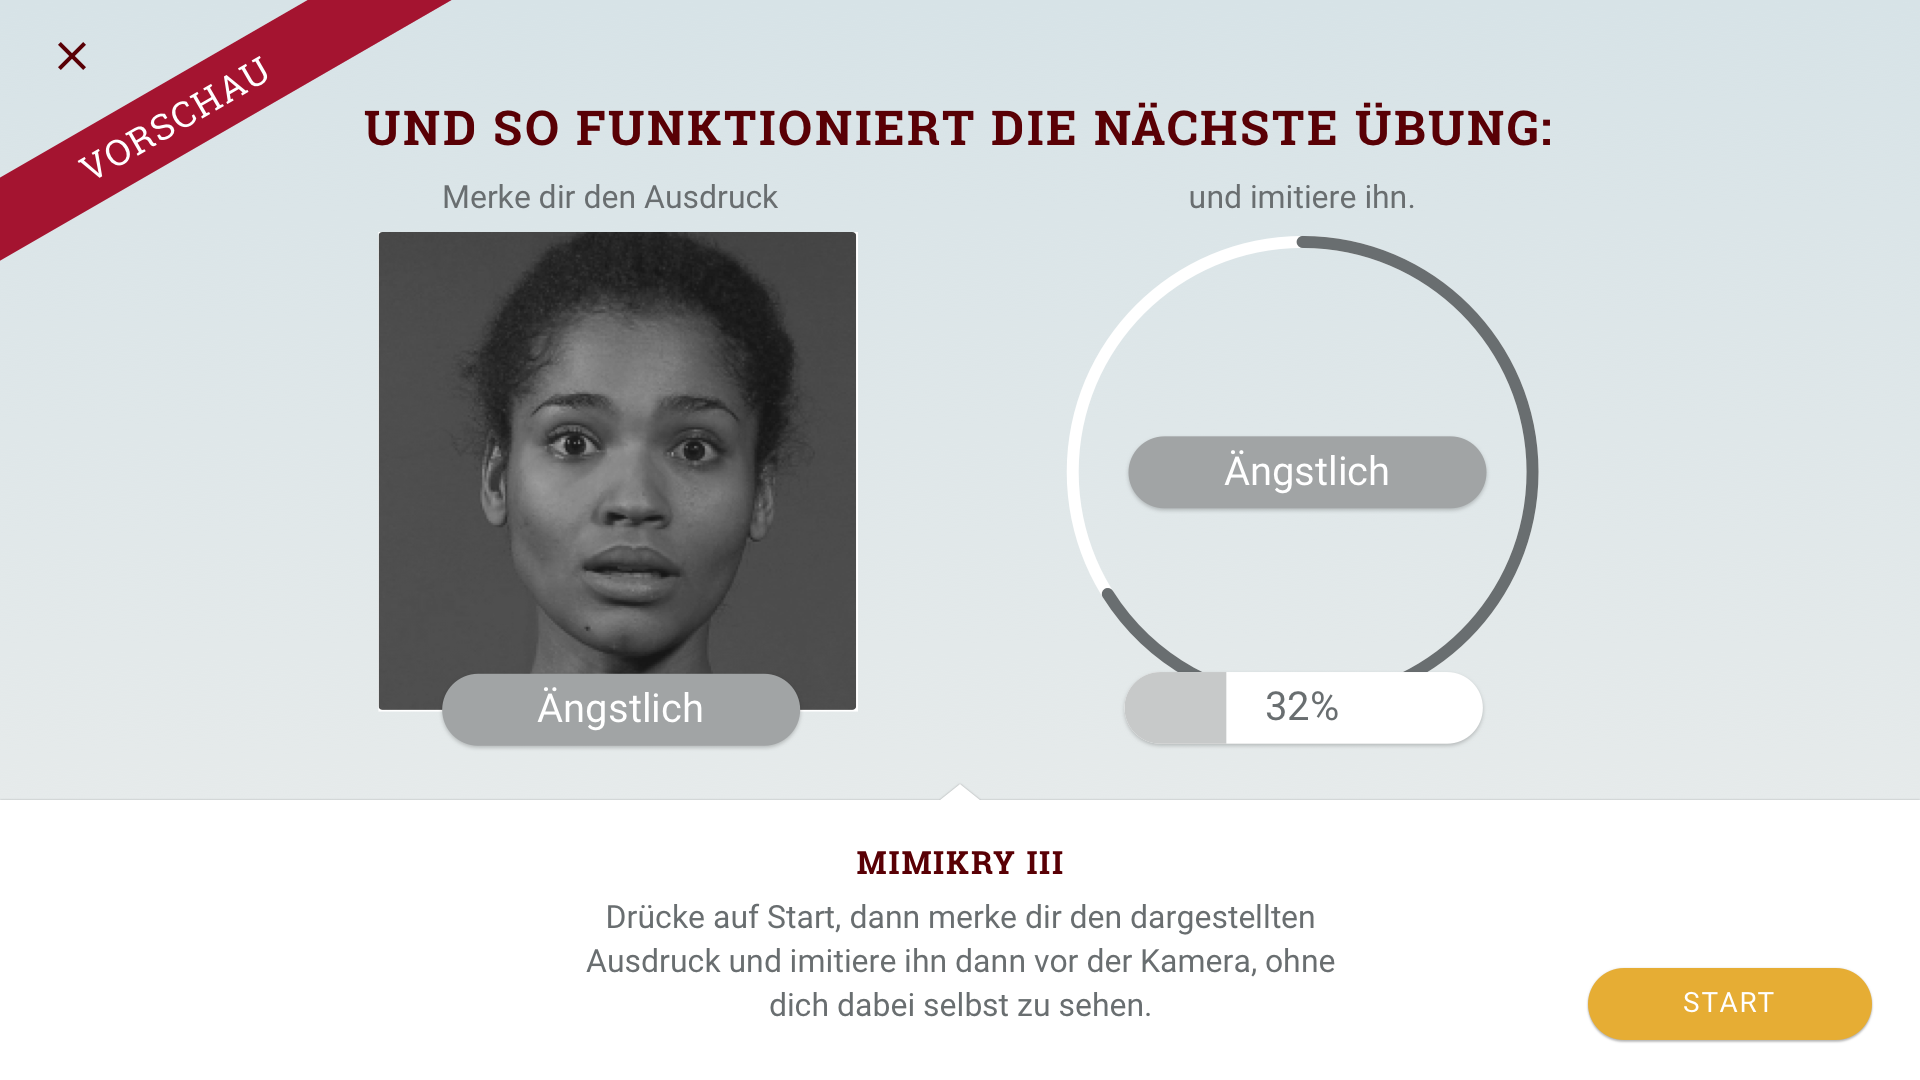
\includegraphics[width=330pt]{res/TASK_MIMIKRY_III_INTRO.png}
\caption{Einführung von Mimikry ohne Vorschau. Das ursprüngliche Mimikry III, wurde während der Implementierung zu Mimikry II umbenannt. 
Die Zielemotion wird auf einem separaten Screen vor dem Anfang einer Aufgabe vermittelt, siehe \ref{knopf}. 
Innerhalb von einem runden Balken befindet sich die Zielemotion, die auf dem vorherigen Screen dargestellt wurde. Darunter befindet sich ein horizontaler, länglicher Balken, der den gegenwärtigen Fortschritt abbilden soll. Die Balken wurden an der Stelle ohne Erklärungspfeilen angezeigt.}
\label{ohne}
\end{figure}
\subsection{Begründung der Auswahl}
Aus folgenden Gründen wurden nur einige der Spielszenarien implementiert, siehe Abb.\ref{reasons} 
\begin{enumerate}
    \item Die zwei Varianten ermöglichen dem Nutzer ein Training und das Ausprobieren des gegenwärtigen Niveaus seiner Mimikry Fähigkeit. Die Stärkung von Mimikry erfolgt durch das wiederholende Trainieren und Erforschen der Mimik bei dem ersten Szenario und durch das Üben der erworbenen Kompetenzen bei dem zweiten Szenario.
    \item Im Rahmen von dem ersten Aufgabetyp sollte der Nutzer seine Gesichtsausdrücke beobachten im Gegensatz zu der zweiten Variante, wo sie nicht angezeigt werden.
    Dieses Vorgehen bei der Auswahl bildet zwei häufigsten Szenarien aus dem Alltagsleben ab
    \item Während der Studie wurden Spielergebnisse gesammelt, die Grundlagen für eine Fortsetzung im Rahmen von einer Bachelor oder Masterarbeit schaffen. Ein Teil der Aufgabenstellung könnte die Implementierung der übrigen Spielszenarien beinhalten.
    \item Die Implementierung aller Varianten würde nicht nur einen Implementierungsaufwand aber auch die Komplexität der Studie deutlich erhöhen.
    \label{reasons}
\end{enumerate}

\subsection{Technische Entscheidungen}
\paragraph{Hardware- und Systemanforderungen.}Die App E.V.A. wurde für Android Geräte mit der Android Version 6 (SDK Version 23, min SDK Version 21) entwickelt. 
SHORE\re wurde für Windows, Linux, Mac OS, Android und ARMv7 entwickelt.
Das Zielgerät ist ein Acer Iconia Tab 10, 10,1 Zoll Full-HD mit 2GB RAM. 
Es wird keine Internetverbindung benötigt, da die Gesichtsanalyse für das Mimikry Modul durch die SHORE\re Software die nur lokal durchgeführt wird. 
\paragraph{Umsetzung der Gesichtsanalyse.}Die technische Umsetzung von dem Emotionserkennung Prozess wurde mittels SHORE\re Gesichtsanalyse Software realisiert. Das Fraunhofer Institut stellte eine Beispiel App zur Verfügung, die auch mit Absprachen im Rahmen von dieser Arbeit weiterentwickelt werden darf. Diese App wird dann in die bereits existierende E.V.A. App als das Mimikry Modul integriert. Im Rahmen der Studie werden zwei Zyklen aus vier Spielen für jede der implementierten Mimikry Varianten. Jedes Spiel beinhaltet eine Einführungsphase, Spielphase mit jeder der Grundemotionen und Feedbackphase nach jedem Spiel. Es werden also insgesamt acht Spiele von jedem Probanden gespielt und jede der Emotion wird in beiden Varianten trainiert.

\paragraph{Datenverwaltung während des Spiels.}Beim Speichern des höchsten erreichten Ergebnisses (in Prozent) der Zielemotion werden die Ergebnisse mittels SharedPreferences, einen Android spezifischen Konzept für kurzfristigen Verwaltung der Daten, gespeichert. Während der Konzeptionsphase wurde das Sammeln von den Spielergebnissen für wissenschaftliche Zwecke, sowie wie eine mögliche Fortsetzung im Rahmen einer Masterarbeit nicht vorgesehen, deswegen wurden die Daten für höchsten erreichten Ergebnisse zusätzlich zu der Datenbank Struktur in SharedPreferences gespeichert. Die Struktur wurde nachträglich angepasst, um es zu ermöglichen.

\paragraph{Das Sammeln von Daten während der Studienphase} wurde abschließend, direkt vor einer UX und Usability Studie mit einer lokalen Datenbank umgesetzt. Die Messungen zur jeder Emotion für jeden Probanden aus jedem der acht Spiele wurden während der Studie gesammelt und in einer lokalen Datenbank anonym gespeichert. Die Datenbank wurde zusätzlich entwickelt, um die zukünftige Fortsetzung der Auseinandersetzung mit der Thematik zu ermöglichen.

\subsection{Anpassungen an dem ursprünglichen Konzept}
Es wurden einige Anpassungen an dem Design und Logik vorgenommen. Gemäß dem ursprünglichen Design sollte der Nutzer eine Möglichkeit haben, ein Foto von sich selbst im Moment des höchsten erreichten Ergebnis speichern zu können. Diese Funktionalität entspricht nicht direkt einem IT-gestützten Mimikry Training. Aufgrund des hohen Implementierungaufwands wurde sie im finalen Konzept des Moduls nicht berücksichtigt. Dadurch wurde die Studie nur für das Abschätzen den für Mimikry relevantesten Spielfragment verantwortlich und ergibt präzisere Ergebnisse über einen Vergleich von zwei alternativen Spielverläufen.
Eine weitere Anpassung lag an der Bestimmung eines Erfolgs oder einer Niederlage beim Lösen einer Aufgabe. Ursprünglich sollte die Aufgabe nach 3 Sekunden von kontinuierlich erreichten Überschreiten einer Schwelle von 75\% bei der Zielemotion als richtig gelöst markiert werden. Da SHORE\re mehrere Ergebnisse pro Sekunde liefert, ist die Wahrscheinlichkeit hoch, dass die ankommenden Messungen auch andere Emotionen innerhalb von diesen 3 Sekunden nachweisen, was sich für das Erreichen des Ziels als sehr anspruchsvoll herausstellte. Aus diesem Grund wurde eine andere Methode gewählt, die genauer in dem Kapitel Implementierung beschrieben wird.
Aufgrund der Auswahl von zwei Szenarien, wurden sie zu Mimikry I und Mimikry II umbenannt.


